
%===================================
%===================================
\section{Comparaciones entre algoritmos}
\label{sec:Comparaciones entre algoritmos}

En esta sección se presentan las comparaciones entre los diferentes algoritmos implementados para la multiplicación de matrices: el algoritmo secuencial, el algoritmo concurrente con hilos, el algoritmo concurrente por procesos y el algoritmo secuencial optimizado por cache line. Se analizarán los tiempos de ejecución y el Speedup obtenido para cada algoritmo en función del tamaño de las matrices utilizadas en las pruebas. Es importante acalarar que en esta comparación solo se hace con los algoritmos que mejor resultado obtienen. A continuación, se muestran las tablas y gráficas correspondientes para comparar el rendimiento de cada algoritmo y discutir los resultados obtenidos.

\begin{figure}[H]
   \centering
   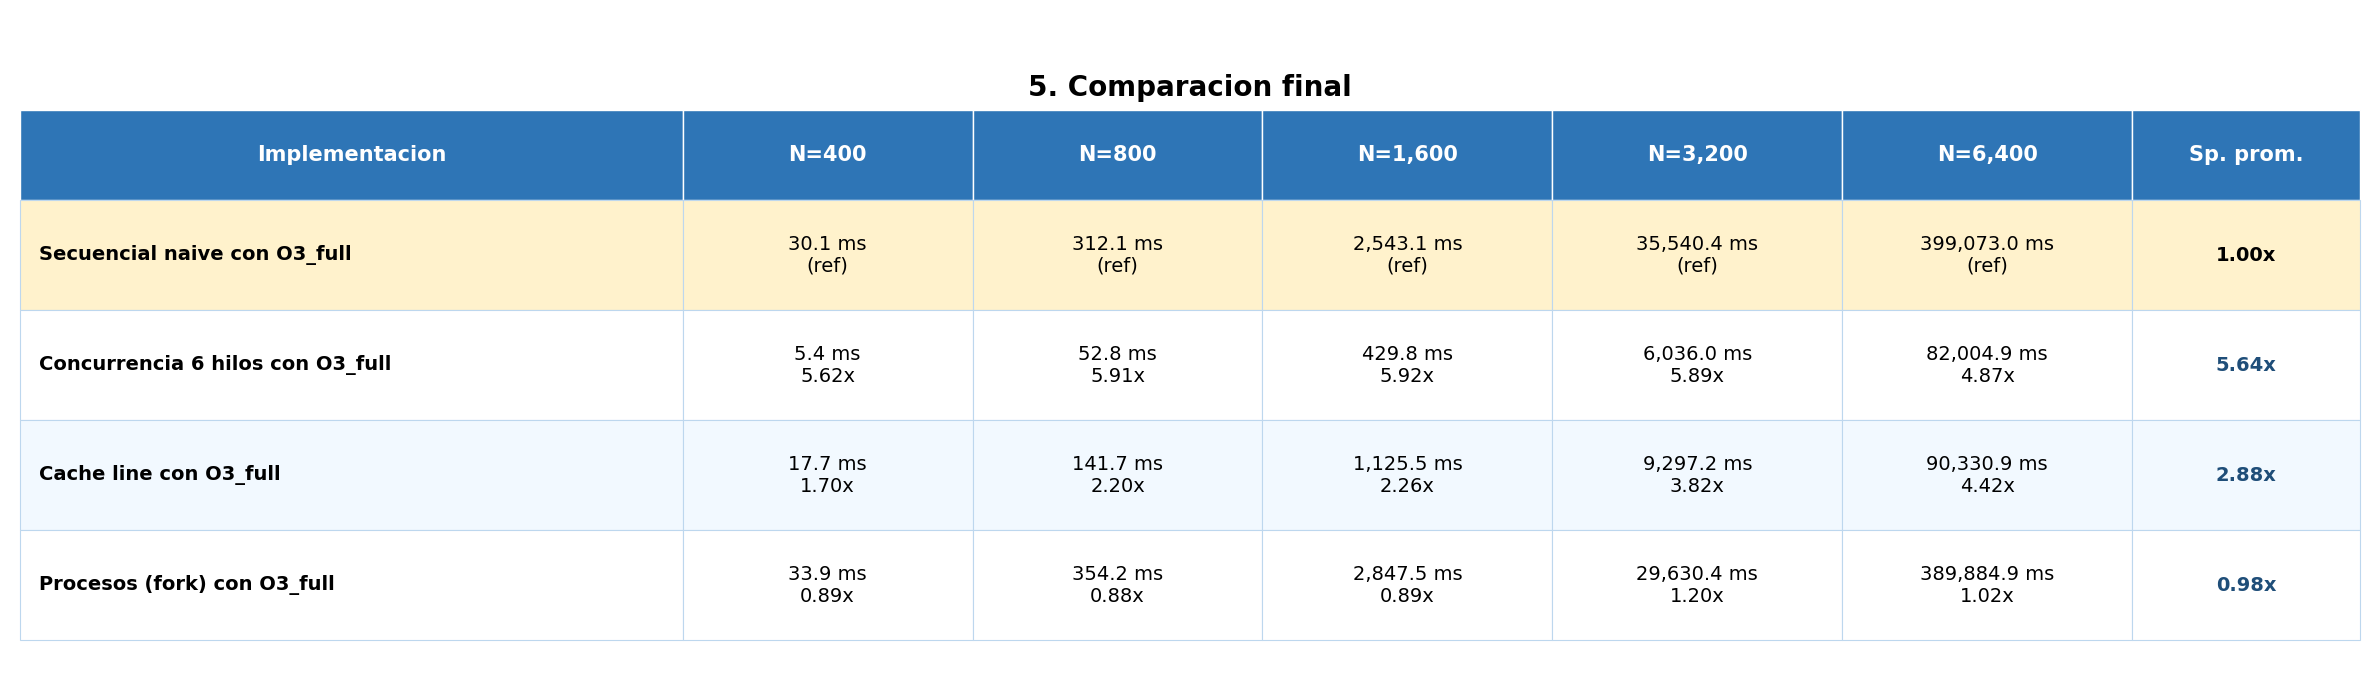
\includegraphics[width=1\textwidth]{images/tables/comparison.png}
   \caption{Tabla de comparación de tiempos de ejecución entre los algoritmos secuencial, concurrente con hilos, concurrente por procesos y secuencial optimizado por cache line.}
   \label{fig:comparison_table}
\end{figure}

\begin{figure}[H]
   \centering
   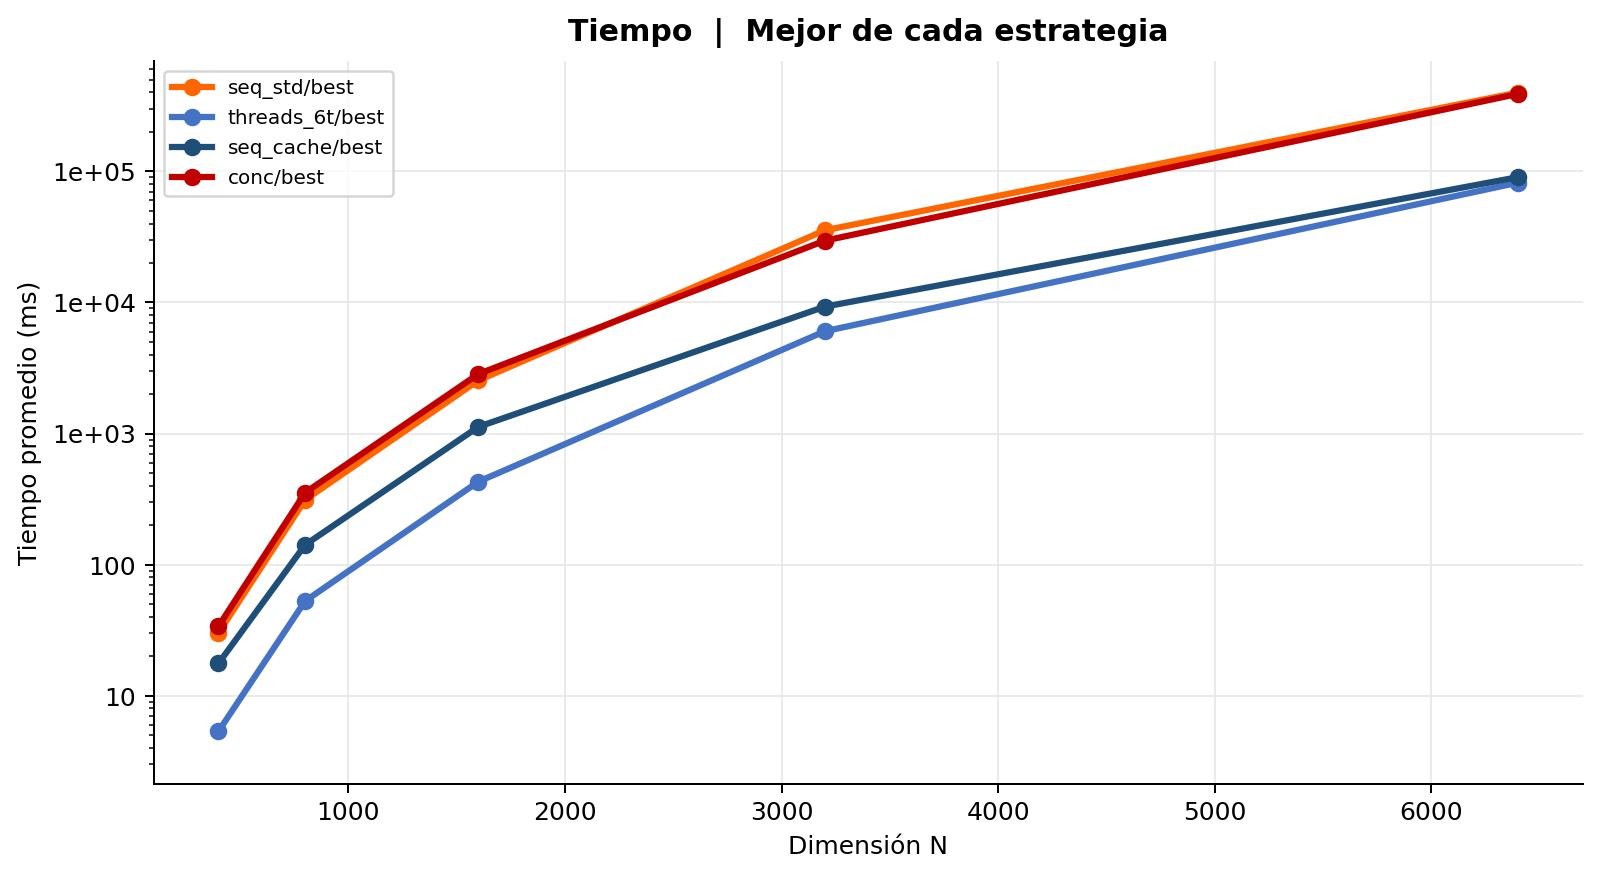
\includegraphics[width=1\textwidth]{images/charts/time_comparison.png}
   \caption{Gráfica de tiempos de ejecución comparativa entre los algoritmos secuencial, concurrente con hilos, concurrente por procesos y secuencial optimizado por cache line.}
   \label{fig:time_comparison}
\end{figure}

\begin{figure}[H]
   \centering
   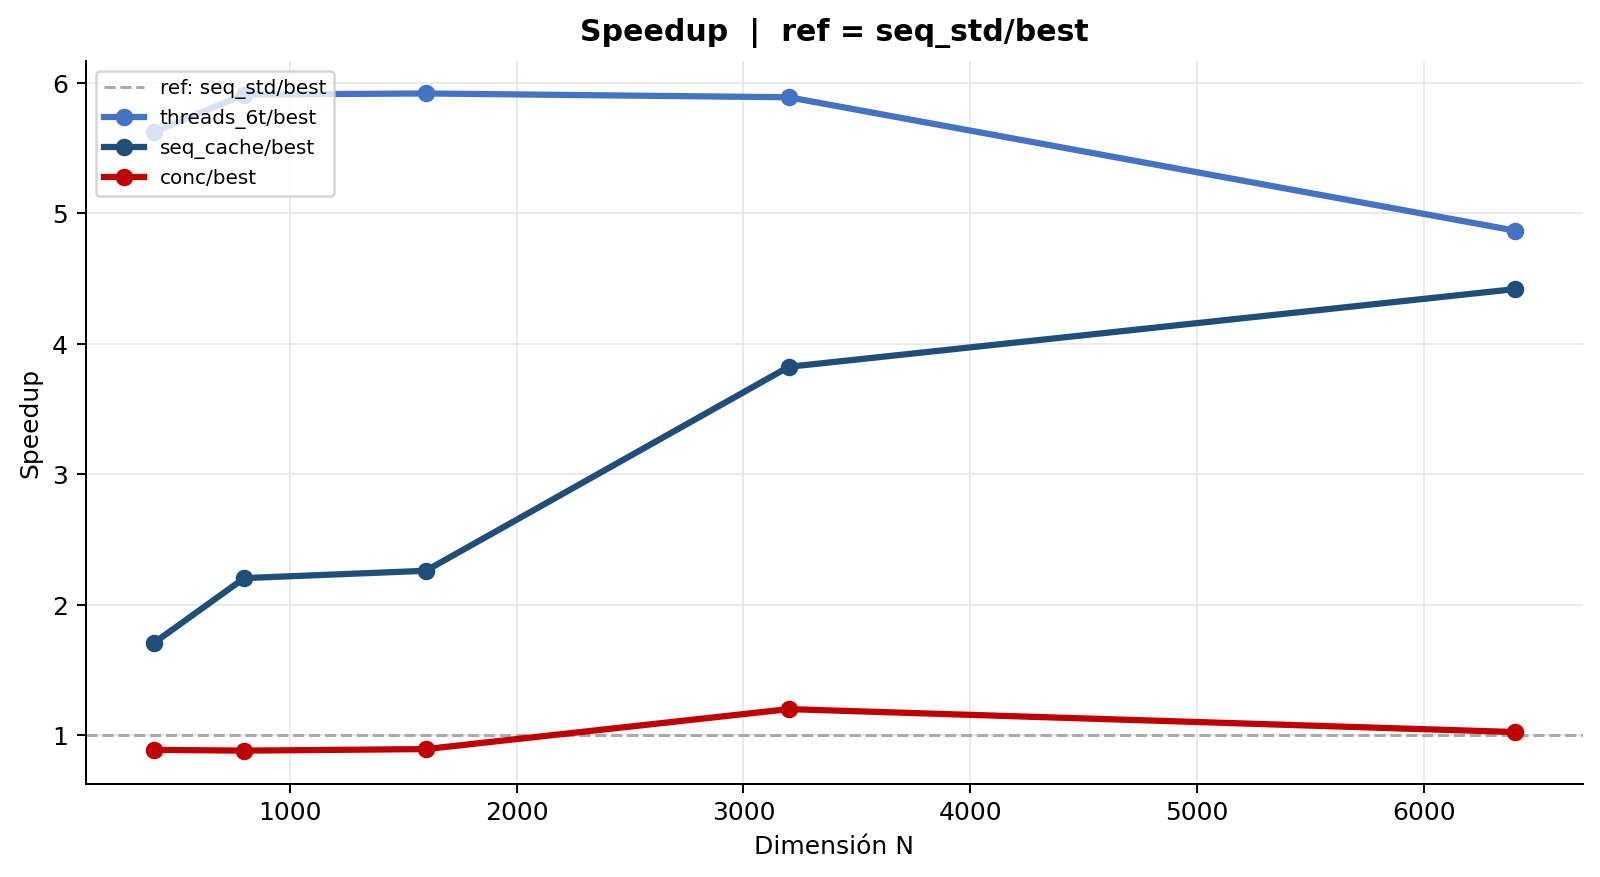
\includegraphics[width=1\textwidth]{images/charts/speedup_comparison.png}
   \caption{Gráfica de Speedup comparativa entre los algoritmos secuencial, concurrente con hilos, concurrente por procesos y secuencial optimizado por cache line.}
   \label{fig:speedup_comparison}
\end{figure}

Observando la tabla del speedup se puede apreciar que el algoritmo concurrente con 6 hilos es el que mayor promedio de speedup tiene, seguido por el algoritmo secuencial optimizado por cache line. El algoritmo concurrente por procesos no muestra una mejora significativa en el rendimiento en comparación con el algoritmo secuencial, lo que sugiere que la sobrecarga de crear y gestionar procesos puede estar afectando negativamente el rendimiento del algoritmo. En general, se puede concluir que el algoritmo concurrente con hilos es el más eficiente para la multiplicación de matrices en este caso, aunque se aprecia una caida de rendimiento en las matrices mas grandes, mientras que el algoritmo secuencial optimizado por cache line también muestra una mejora en el rendimiento.
   